\documentclass[border=4pt]{standalone}
\usepackage[utf8]{inputenc}
\usepackage[T1]{fontenc}
\usepackage{lmodern}
\usepackage{amsmath,amssymb,mathtools}
\usepackage{tikz}
\usetikzlibrary{calc,decorations.pathreplacing,angles,quotes}
\usepackage{pgfplots}
\pgfplotsset{compat=1.18}
% Figura extraída de la Tarea 11 de Cálculo I (primer semestre).
\begin{document}
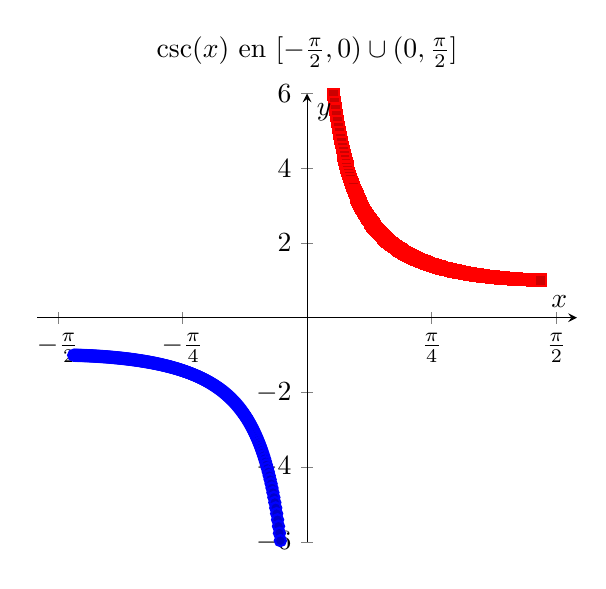
\begin{tikzpicture}
        \begin{axis}[
        domain=-1.4708:1.4708,samples=250,
        xmin=-1.7,xmax=1.7,ymin=-6,ymax=6,
        axis lines=middle,xlabel={$x$},ylabel={$y$},
        xtick={-1.5708,-0.7854,0,0.7854,1.5708},
        xticklabels={\(-\tfrac{\pi}{2}\),\(-\tfrac{\pi}{4}\),0,\(\tfrac{\pi}{4}\),\(\tfrac{\pi}{2}\)},
        title={\(\csc(x)\) en \([-\tfrac{\pi}{2},0)\cup(0,\tfrac{\pi}{2}]\)}
        ]
        \addplot+[thick,domain=-1.4708:-0.01]{1/sin(deg(x))};
        \addplot+[thick,domain=0.01:1.4708]{1/sin(deg(x))};
        \draw[dashed](axis cs:0,-6)--(axis cs:0,6);
        \end{axis}
    \end{tikzpicture}
\end{document}
